\documentclass[tikz,border=10mm]{standalone}
\usepackage{helvet}
\renewcommand{\familydefault}{\sfdefault}
\usepackage{tikz}
\usetikzlibrary{arrows.meta, positioning, fit, calc, decorations.pathreplacing, backgrounds}

% Define colors
\definecolor{emeraldpine}{HTML}{1A4D3E}
\definecolor{harvardcrimson}{HTML}{A51C30}
\definecolor{ethdarkblue}{HTML}{1F407A}
\definecolor{ethpetrol}{HTML}{007A87}
\definecolor{ethbronze}{HTML}{B87333}
\definecolor{ink}{HTML}{1A202C}
\definecolor{softink}{HTML}{4A5568}
\definecolor{paleink}{HTML}{A0AEC0}
\definecolor{cardbg}{HTML}{F8FAFC}
\definecolor{shadecolor}{HTML}{F4F6F9}

\begin{document}
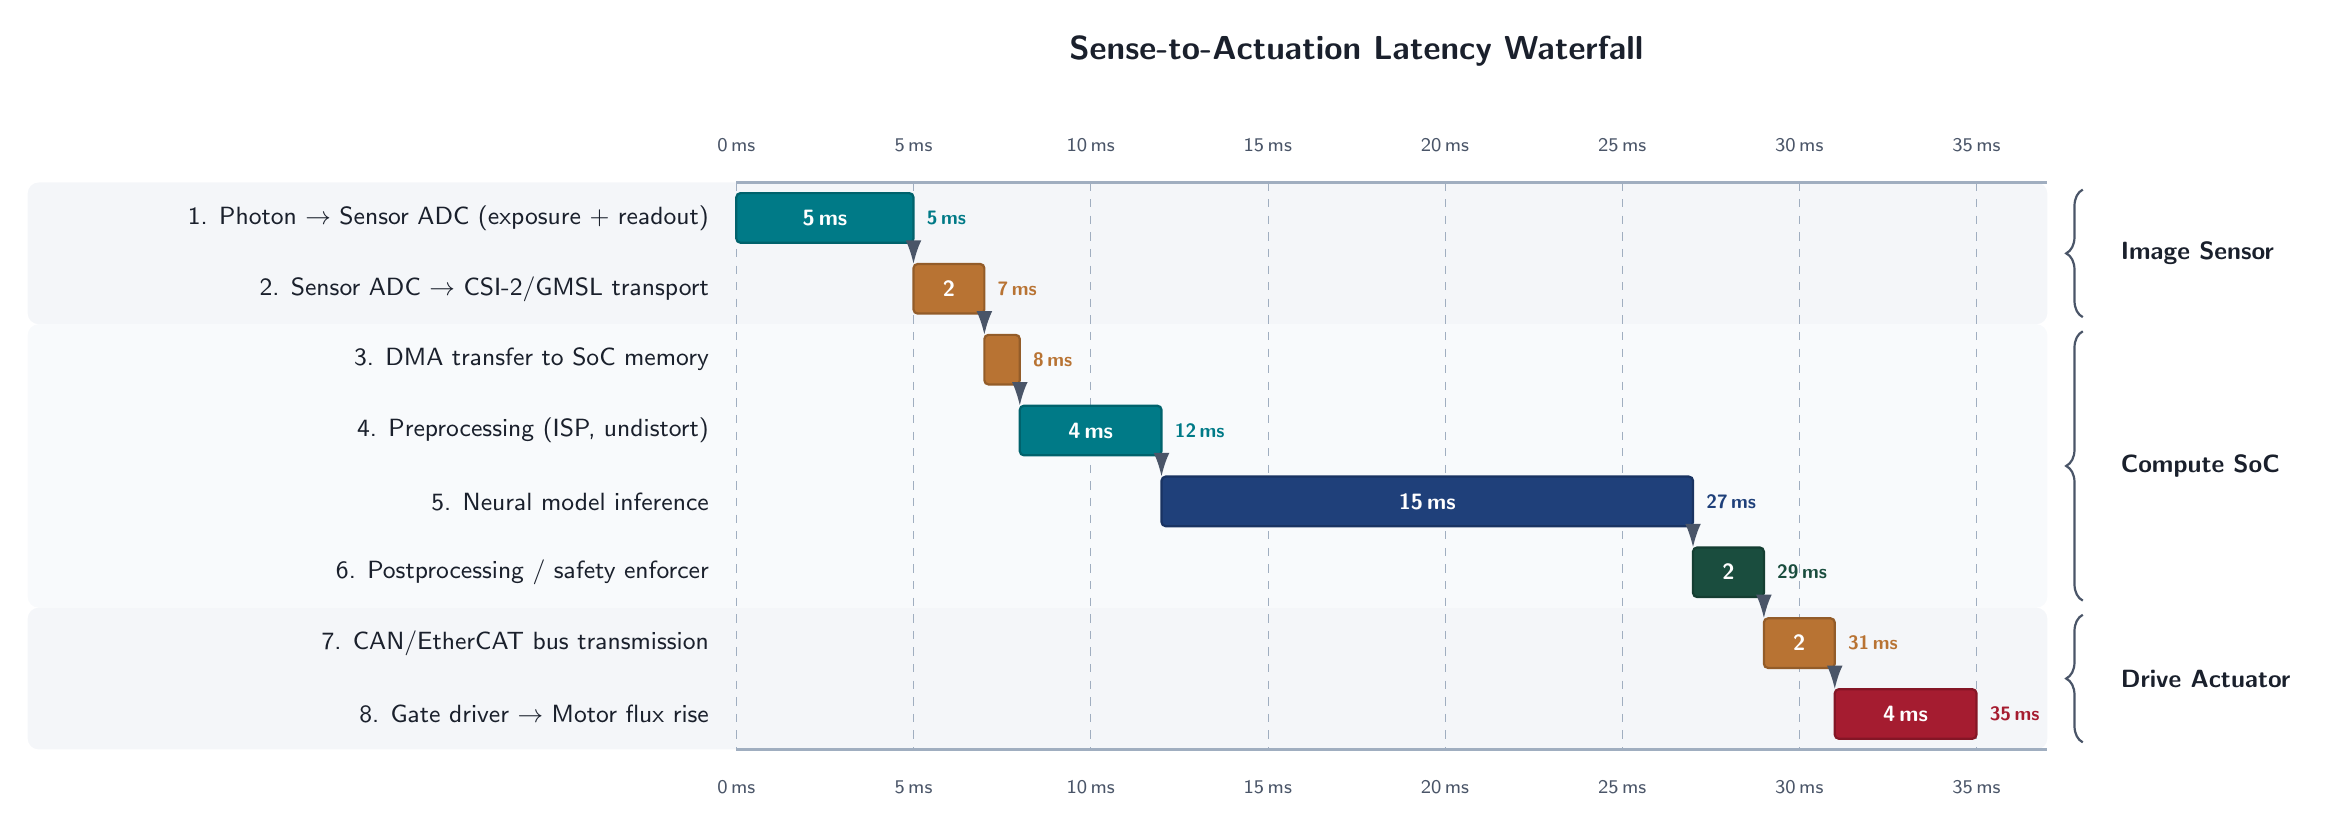
\begin{tikzpicture}[x=4.5mm, y=-9mm, font=\sffamily]

% Draw background grouping boxes first
\fill[shadecolor, rounded corners=4pt] (-20, 0.5) rectangle (37, 2.5);
\fill[cardbg, rounded corners=4pt] (-20, 2.5) rectangle (37, 6.5);
\fill[shadecolor, rounded corners=4pt] (-20, 6.5) rectangle (37, 8.5);

% Grid lines and X-axis
\foreach \x in {0, 5, 10, 15, 20, 25, 30, 35} {
    \draw[paleink, very thin, dashed] (\x, 0.5) -- (\x, 8.5);
    \node[softink, anchor=south, font=\scriptsize] at (\x, 0.2) {\x\,ms};
    \node[softink, anchor=north, font=\scriptsize] at (\x, 8.8) {\x\,ms};
}
\draw[paleink, thick] (0, 0.5) -- (37, 0.5);
\draw[paleink, thick] (0, 8.5) -- (37, 8.5);

% Title
\node[ink, anchor=south, font=\bfseries\large] at (17.5, -1) {Sense-to-Actuation Latency Waterfall};

% Define macro for stage
\newcommand{\waterfallstage}[7]{
    \fill[#4, rounded corners=1.5pt] (#1, #3-0.35) rectangle ++(#2, 0.7);
    \draw[#4!80!black, thick, rounded corners=1.5pt] (#1, #3-0.35) rectangle ++(#2, 0.7);
    \node[ink, anchor=east, font=\small] at (-0.5, #3) {#7};
}

% 1. Exposure: 5 ms
\waterfallstage{0}{5}{1}{ethpetrol}{}{5}{1. Photon $\rightarrow$ Sensor ADC (exposure + readout)};
\node[white, font=\footnotesize\bfseries] at (2.5, 1) {5\,ms};
\node[ethpetrol, anchor=west, font=\scriptsize\bfseries] at (5.1, 1) {5\,ms};

% 2. CSI-2 transport: 2 ms
\waterfallstage{5}{2}{2}{ethbronze}{}{7}{2. Sensor ADC $\rightarrow$ CSI-2/GMSL transport};
\node[white, font=\footnotesize\bfseries] at (6, 2) {2};
\node[ethbronze, anchor=west, font=\scriptsize\bfseries] at (7.1, 2) {7\,ms};

% 3. DMA: 1 ms
\waterfallstage{7}{1}{3}{ethbronze}{}{8}{3. DMA transfer to SoC memory};
\node[ethbronze, anchor=west, font=\scriptsize\bfseries] at (8.1, 3) {8\,ms};

% 4. Preprocessing: 4 ms
\waterfallstage{8}{4}{4}{ethpetrol}{}{12}{4. Preprocessing (ISP, undistort)};
\node[white, font=\footnotesize\bfseries] at (10, 4) {4\,ms};
\node[ethpetrol, anchor=west, font=\scriptsize\bfseries] at (12.1, 4) {12\,ms};

% 5. Inference: 15 ms
\waterfallstage{12}{15}{5}{ethdarkblue}{}{27}{5. Neural model inference};
\node[white, font=\footnotesize\bfseries] at (19.5, 5) {15\,ms};
\node[ethdarkblue, anchor=west, font=\scriptsize\bfseries] at (27.1, 5) {27\,ms};

% 6. Safety enforcer: 2 ms
\waterfallstage{27}{2}{6}{emeraldpine}{}{29}{6. Postprocessing / safety enforcer};
\node[white, font=\footnotesize\bfseries] at (28, 6) {2};
\node[emeraldpine, anchor=west, font=\scriptsize\bfseries] at (29.1, 6) {29\,ms};

% 7. Bus transmission: 2 ms
\waterfallstage{29}{2}{7}{ethbronze}{}{31}{7. CAN/EtherCAT bus transmission};
\node[white, font=\footnotesize\bfseries] at (30, 7) {2};
\node[ethbronze, anchor=west, font=\scriptsize\bfseries] at (31.1, 7) {31\,ms};

% 8. Motor flux rise: 4 ms
\waterfallstage{31}{4}{8}{harvardcrimson}{}{35}{8. Gate driver $\rightarrow$ Motor flux rise};
\node[white, font=\footnotesize\bfseries] at (33, 8) {4\,ms};
\node[harvardcrimson, anchor=west, font=\scriptsize\bfseries] at (35.1, 8) {35\,ms};

% Silicon Boundaries on the right
\draw[decorate, decoration={brace, amplitude=6pt, mirror}, thick, softink] (38, 0.6) -- (38, 2.4) node[midway, right=10pt, font=\bfseries\small, text=ink] {Image Sensor};
\draw[decorate, decoration={brace, amplitude=6pt, mirror}, thick, softink] (38, 2.6) -- (38, 6.4) node[midway, right=10pt, font=\bfseries\small, text=ink] {Compute SoC};
\draw[decorate, decoration={brace, amplitude=6pt, mirror}, thick, softink] (38, 6.6) -- (38, 8.4) node[midway, right=10pt, font=\bfseries\small, text=ink] {Drive Actuator};

% Add connecting casual arrows between stages (waterfall steps)
\draw[-{Latex[length=3mm, width=2mm]}, softink, thick] (5, 1.35) -- (5, 1.65);
\draw[-{Latex[length=3mm, width=2mm]}, softink, thick] (7, 2.35) -- (7, 2.65);
\draw[-{Latex[length=3mm, width=2mm]}, softink, thick] (8, 3.35) -- (8, 3.65);
\draw[-{Latex[length=3mm, width=2mm]}, softink, thick] (12, 4.35) -- (12, 4.65);
\draw[-{Latex[length=3mm, width=2mm]}, softink, thick] (27, 5.35) -- (27, 5.65);
\draw[-{Latex[length=3mm, width=2mm]}, softink, thick] (29, 6.35) -- (29, 6.65);
\draw[-{Latex[length=3mm, width=2mm]}, softink, thick] (31, 7.35) -- (31, 7.65);

\end{tikzpicture}
\end{document}
